\documentclass[a4paper]{article}
\usepackage{geometry}
\usepackage{graphicx}
\usepackage{natbib}
\usepackage{amsmath}
\usepackage{amssymb}
\usepackage{amsthm}
\usepackage{paralist}
\usepackage{epstopdf}
\usepackage{tabularx}
\usepackage{longtable}
\usepackage{multirow}
\usepackage{multicol}
\usepackage[hidelinks]{hyperref}
\usepackage{fancyvrb}
\usepackage{algorithm}
\usepackage{algorithmic}
\usepackage{float}
\usepackage{paralist}
\usepackage[svgname]{xcolor}
\usepackage{enumerate}
\usepackage{array}
\usepackage{times}
\usepackage{url}
\usepackage{fancyhdr}
\usepackage{comment}
\usepackage{environ}
\usepackage{times}
\usepackage{textcomp}
\usepackage{caption}
\usepackage{listings}

\urlstyle{rm}

\setlength\parindent{0pt} % Removes all indentation from paragraphs
\theoremstyle{definition}
\newtheorem{definition}{Definition}[]
\newtheorem{conjecture}{Conjecture}[]
\newtheorem{example}{Example}[]
\newtheorem{theorem}{Theorem}[]
\newtheorem{lemma}{Lemma}
\newtheorem{proposition}{Proposition}
\newtheorem{corollary}{Corollary}

\floatname{algorithm}{Procedure}
\renewcommand{\algorithmicrequire}{\textbf{Input:}}
\renewcommand{\algorithmicensure}{\textbf{Output:}}
\newcommand{\abs}[1]{\lvert#1\rvert}
\newcommand{\norm}[1]{\lVert#1\rVert}
\newcommand{\RR}{\mathbb{R}}
\newcommand{\CC}{\mathbb{C}}
\newcommand{\Nat}{\mathbb{N}}
\newcommand{\br}[1]{\{#1\}}
\DeclareMathOperator*{\argmin}{arg\,min}
\DeclareMathOperator*{\argmax}{arg\,max}
\renewcommand{\qedsymbol}{$\blacksquare$}

\definecolor{dkgreen}{rgb}{0,0.6,0}
\definecolor{gray}{rgb}{0.5,0.5,0.5}
\definecolor{mauve}{rgb}{0.58,0,0.82}

\newcommand{\Var}{\mathrm{Var}}
\newcommand{\Cov}{\mathrm{Cov}}

\newcommand{\vc}[1]{\boldsymbol{#1}}
\newcommand{\xv}{\vc{x}}
\newcommand{\Sigmav}{\vc{\Sigma}}
\newcommand{\alphav}{\vc{\alpha}}
\newcommand{\muv}{\vc{\mu}}

\newcommand{\red}[1]{\textcolor{red}{#1}}

\def\x{\mathbf x}
\def\y{\mathbf y}
\def\w{\mathbf w}
\def\v{\mathbf v}
\def\E{\mathbb E}
\def\V{\mathbb V}

% TO SHOW SOLUTIONS, include following (else comment out):
\newenvironment{soln}{
    \leavevmode\color{blue}\ignorespaces
}{}


\hypersetup{
%    colorlinks,
    linkcolor={red!50!black},
    citecolor={blue!50!black},
    urlcolor={blue!80!black}
}

\geometry{
  top=1in,            % <-- you want to adjust this
  inner=1in,
  outer=1in,
  bottom=1in,
  headheight=3em,       % <-- and this
  headsep=2em,          % <-- and this
  footskip=3em,
}


\pagestyle{fancyplain}
\lhead{\fancyplain{}{Homework 2}}
\rhead{\fancyplain{}{CS 760 Machine Learning}}
\cfoot{\thepage}

\title{\textsc{Homework 2}} % Title

%%% NOTE:  Replace 'NAME HERE' etc., and delete any "\red{}" wrappers (so it won't show up as red)

\author{
\red{Deepan Das} \\
\red{ddas27}\\
} 

\date{}

\begin{document}

\maketitle 


\textbf{Instructions:} 
Although this is a programming homework, you only need to hand in a pdf answer file.
There is no need to submit the latex source or any code.
You can choose any programming language, as long as you implement the algorithm from scratch (e.g. do not use Weka on questions 1 to 7).  

Use this latex file as a template to develop your homework.
Submit your homework on time as a single pdf file to Canvas.
Please check Piazza for updates about the homework.

\section{A Simplified Decision Tree}
You are to implement a decision-tree learner for classification.
To simplify your work, this will not be a general purpose decision tree.  Instead, your program can assume that
\begin{itemize}
\item each item has two continuous features $\x \in \RR^2$
\item the class label is binary and encoded as $y \in \{0,1\}$
\item data files are in plaintext with one labeled item per line, separated by whitespace:
$$x_{11} \quad x_{12} \quad y_1$$
$$...$$
$$x_{n1} \quad x_{n2} \quad y_n$$
\end{itemize}

Your program should implement a decision tree learner according to the following guidelines:
\begin{itemize}
\item Candidate splits $(j,c)$ for numeric features should use a threshold $c$ in feature dimension $j$ in the form of $x_{\cdot j}\ge c$.
\item $c$ should be on values of that dimension present in the training data; i.e. the threshold is on training points, not in between training points.
\item The left branch of such a split is the ``then'' branch, and the right branch is ``else''.
\item Splits should be chosen using mutual information (i.e. information gain). If there is a tie you may break it arbitrarily.
\item The stopping criteria (for making a node into a leaf) are that 
	\begin{itemize}
	\item the node is empty, or
	\item all splits have zero mutual information
	\end{itemize}
\item To simplify, whenever there is no majority class in a leaf, let it predict $y=1$.
\end{itemize}

\section{Questions}
\begin{enumerate}
\item (Our algorithm stops at pure labels) [10 pts] If a node is not empty but contains training items with the same label, why is it guaranteed to become a leaf?  Explain.


\begin{soln}  

In such a setup, where we have one non-empty node, but with training items of the same label(let's assume predicted label = $0$) we have two options at hand:
\begin{itemize}
	\item Hypothesis $H_{1}$: Stop determining any further splits from that node
	\item Hypothesis $H_{2}$: Determine a set of thresholds at this node $n$, $C_n = {c_1, c_2, ... ,c_n} $ such that there are splits determined at each of these thresholds, and the label is always $0$ for each such split. Furthermore, let's assume there are $a_1, a_2, a_3, ..., a_n$ elements for each such split, such that $a_1 + a_2 + ... + a_n = A_n$, where $A_n$ is the number of elements remaining at node $n$ and have the same label $0$.
\end{itemize}

Now, Entropy at node $n$: 
$$
\mathbf{E(n, A_n) = - p_1 log(p_1) - p_0 log(p_0) = -0*log(0) - 1*log(1) = 0}
$$


Entropy at any subsplit $c_i$
$$
\mathbf{E(c_i, a_i) = - p_1 log(p_1) - p_0 log(p_0) = -0*log(0) - 1*log(1) = 0}
$$

Average Entropy of  all $n$ sub-splits due to threshold-set $C$ is:

$$
\mathbf{E(C, A_n) = \frac{a_1}{A_n} E(c_1, a_1) + \frac{a_2}{A_n} E(c_2, a_2) + ... + \frac{a_n}{A_n} E(c_n, a_n) = 0 + 0 + ... + 0 = 0}
$$

Thus, information gain: 
$$
\mathbf{E(n, A_n) - E(C, A_n) = 0}
$$

Thus, there are two reasons to stop at this stage itself and not go further.

\begin{itemize}
	\item We see that all splits from this point have zero mutual information, which is a stopping criteria.
	\item Simply by Occam's razor, we should choose one amongst the two competing hypotheses that make exactly the same predictions, and the chosen one should be the simpler one, which is $H_1$ in this case, and thus, not split any further.
\end{itemize}


\end{soln}

\item (Our algorithm is greedy)  [10 pts] Handcraft a small training set where both classes are present but the algorithm refuses to split; instead it makes the root a leaf and stop;
Importantly, if we were to manually force a split, the algorithm will happily continue splitting the data set further and produce a deeper tree with zero training error.
You should (1) plot your training set, (2) explain why.  Hint: you don't need more than a handful of items. 
	   % \begin{figure}[H]
	   %     \centering
	   %     \includegraphics[width=0.4\textwidth]{FIGURE_FILENAME.pdf}
	   %     \captionsetup{labelformat=empty}
	   %     \caption{}
	   %     \label{fig:my_label}
	   % \end{figure}
	   
\begin{soln}
	Lets consider the following dataset: 
	\begin{center}
		\begin{tabular}{ c c c }
			x1 & x2 & outcome \\
			0 & 0 & 0 \\ 
			0 & 1 & 1 \\
			1 & 0 & 1 \\
			1 & 1 & 0  
		\end{tabular}
	\end{center}

The dataset scatter plot looks like this:
 \begin{figure}[H]
     \centering
     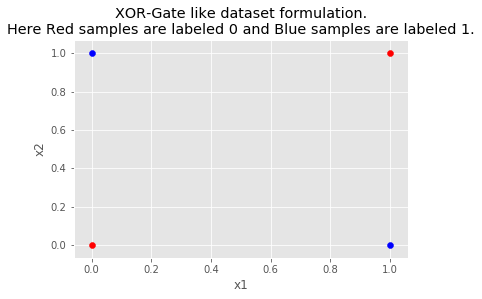
\includegraphics[width=0.7\textwidth]{q2.png}
     \captionsetup{labelformat=empty}
     \caption{}
     \label{fig:my_label}
 \end{figure}

Now, initial entropy for this dataset is: 

$$
\mathbf{E_0 = -p_0 log(p_0) - p_1 log(p_1) = - 0.5 * log(0.5) - 0.5 * log(0.5) = 1.0}
$$

Now, let's consider the split where $x1 >= 1$. The Entropy for the two splits due to this condition also turns out to be:

$$ E_{S1, x1>=1} = 1.0 and E_{S2,x1<1}  = 1.0 $$

Also, considering other split conditions like $x2 >= 1$ leads to similar results in individual split entropies. Under such a condition we note that no split is able to provide any information gain, i.e. Information gain is $0$. Thus, we arrive at a stopping criteria and the decision tree stops at the head node itself and assigns everything a random label($1$ in our case).

However, if we can manually set some rules, we can easily assign a label to each datapoint. The rules would be: 


	$\mathbf{ x1 >= 1 \hspace{0.5cm} \& \hspace{0.5cm}x2 >= 1: assign 0} $\\
	$\mathbf{ x1 >= 1 \hspace{0.5cm}\& \hspace{0.5cm}x2 < 1: assign 1}$ \\
	$\mathbf{ x1 < 1 \hspace{0.5cm}\& \hspace{0.5cm}x2 >= 1: assign 1}$ \\
	$\mathbf{ x1 < 1 \hspace{0.5cm}\& \hspace{0.5cm}x2 < 1: assign 0}$

Thus, the stopping criteria of having zero information gain essentially doesn't let the tree split further, as there is no correlation between any attribute and labels. But, we can set explicit conditions manually that can divide the feature space minutely and accordingly. 



\end{soln}

\item (Mutual information exercise)  [10 pts] Use the training set Druns.txt.  For the root node, list all candidate cuts and their mutual information.  Hint: to get $\log_2(x)$ when your programming language may be using a different base, use \verb|log(x)/log(2)|.

\begin{soln}
	
	
	The candidate splits and the information gain is listed in the following table:
	
		\begin{center}
		\begin{tabular}{ c c }
			condition & Information Gain \\
			x1 $\geq$ 0.1 & 0.0315 \\ 
			x1 $\geq$ 0  & 0 \\
			x2 $\geq$ -2.0 & 0 \\
			x2 $\geq$ -1.0 & 0.0315 \\
			x2 $\geq$ 0.0 & -0.0341 \\
			x2 $\geq$ 1.0 & -0.0428 \\
			x2 $\geq$ 2.0 & -0.0395 \\
			x2 $\geq$ 3.0 & -0.0299 \\
			x2 $\geq$ 4.0 & -0.0148 \\
			x2 $\geq$ 5.0 & 0.0062 \\
			x2 $\geq$ 6.0 & 0.0401 \\
			x2 $\geq$ 7.0 & -0.0341 \\
			x2 $\geq$ 8.0 & 0.1042 \\			
		\end{tabular}
	\end{center}
	
The resulting tree then looks like the following:
 \begin{figure}[H]
	\centering
	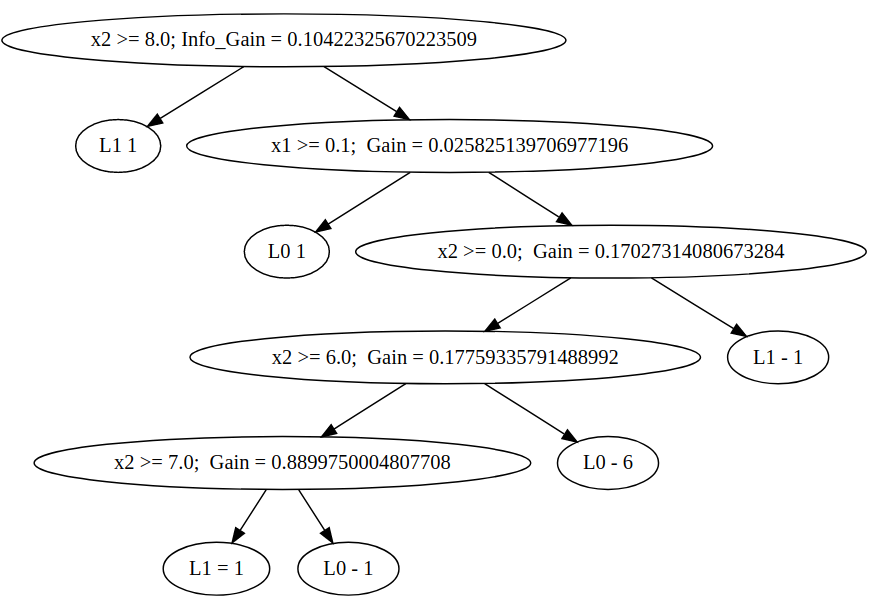
\includegraphics[width=0.7\textwidth]{Druns_tree.png}
	\captionsetup{labelformat=empty}
	\caption{}
	\label{fig:my_label}
\end{figure}

\end{soln}

\item (The king of interpretability)  [10 pts] Decision tree is not the most accurate classifier in general.  However, it persists.  This is largely due to its rumored interpretability: a data scientist can easily explain a tree to a non-data scientist.  Build a tree from D3leaves.txt.  Then manually convert your tree to a set of logic rules.  Show the tree\footnote{When we say show the tree, we mean either the standard computer science tree view, or some crude plaintext representation of the tree -- as long as you explain the format.  When we say visualize the tree, we mean a plot in the 2D $\x$ space that shows how the tree will classify any points.} and the rules.


\begin{soln}
	The tree built from D3leaves.txt is as follows:
	In the tree visualization, each leaf node has its label as $L1 or L0$. The number of instances in each lead node is mentioned alongwith it. In each split node, the attribute condition is mentioned along with the information gain obtained because of that.

 \begin{figure}[H]
	\centering
	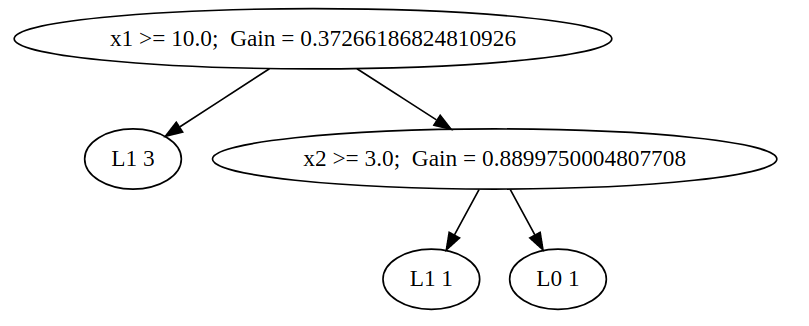
\includegraphics[width=0.7\textwidth]{D3leaves_tree.png}
	\captionsetup{labelformat=empty}
	\caption{}
	\label{fig:my_label}
\end{figure}

The logic rules for the above tree can be summarized as:

\begin{lstlisting}

If x1 >= 10:
    assign label 1
else:
    If x2 >= 3:
        assign label 1
    else:
    	assign label 0  
	
\end{lstlisting}
	
	
	
\end{soln}



\item (Or is it?)  [20 pts] For this question only, make sure you DO NOT VISUALIZE the data sets or plot your tree's decision boundary in the 2D $\x$ space.  If your code does that, turn it off before proceeding.  This is because you want to see your own reaction when trying to interpret a tree.  You will get points no matter what your interpretation is.
And we will ask you to visualize them in the next question anyway.
  \begin{itemize}
  \item Build a decision tree on D1.txt.  Show it to us in any format (e.g. could be a standard binary tree with nodes and arrows, and denote the rule at each leaf node; or Weka style plaintext tree; or as simple as plaintext output where each line represents a node with appropriate line number pointers to child nodes; whatever is convenient for you). Again, do not visualize the data set or the tree in the $\x$ input space.  In real tasks you will not be able to visualize the whole high dimensional input space anyway, so we don't want you to ``cheat'' here.
  
  \begin{soln}
  	The decision tree looks like the following: 
  	
  	 \begin{figure}[H]
  		\centering
  		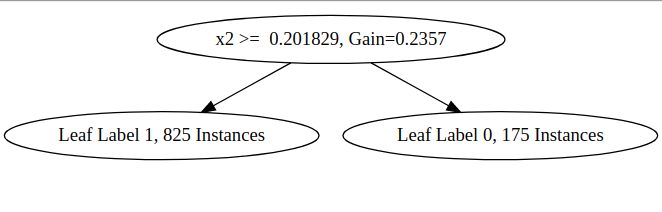
\includegraphics[width=0.7\textwidth]{D1_tree.png}
  		\captionsetup{labelformat=empty}
  		\caption{}
  		\label{fig:my_label}
  	\end{figure}
  	
  	
  \end{soln}
  
  
  \item Look at your tree in the above format (remember, you should not visualize the 2D dataset or your tree's decision boundary) and try to interpret the decision boundary in human understandable English. 
  
  \begin{soln}
  	The decision tree basically is able to correctly model the training data on the basis of one threshold in the $x2$ dimension. The decision tree suggests that all datapoints whose attribute $x2 \geq 0.201829$, they are assigned label 1 and there are 825 such instances. On the other hand, when $x2 \le 0.201829$, all datapoints are labeled 0. Since, decision trees form decision boundaries form decision boundaries parallel to the axes, and since there's only one decision point, we can assume there is a single continuous decision boundary parallel to the X-axis. 
  \end{soln}
  
  \item Build a decision tree on D2.txt.  Show it to us.
  
  \begin{soln}
  	The decision tree looks like the following: 
  	
  	\begin{figure}[H]
  		\centering
  		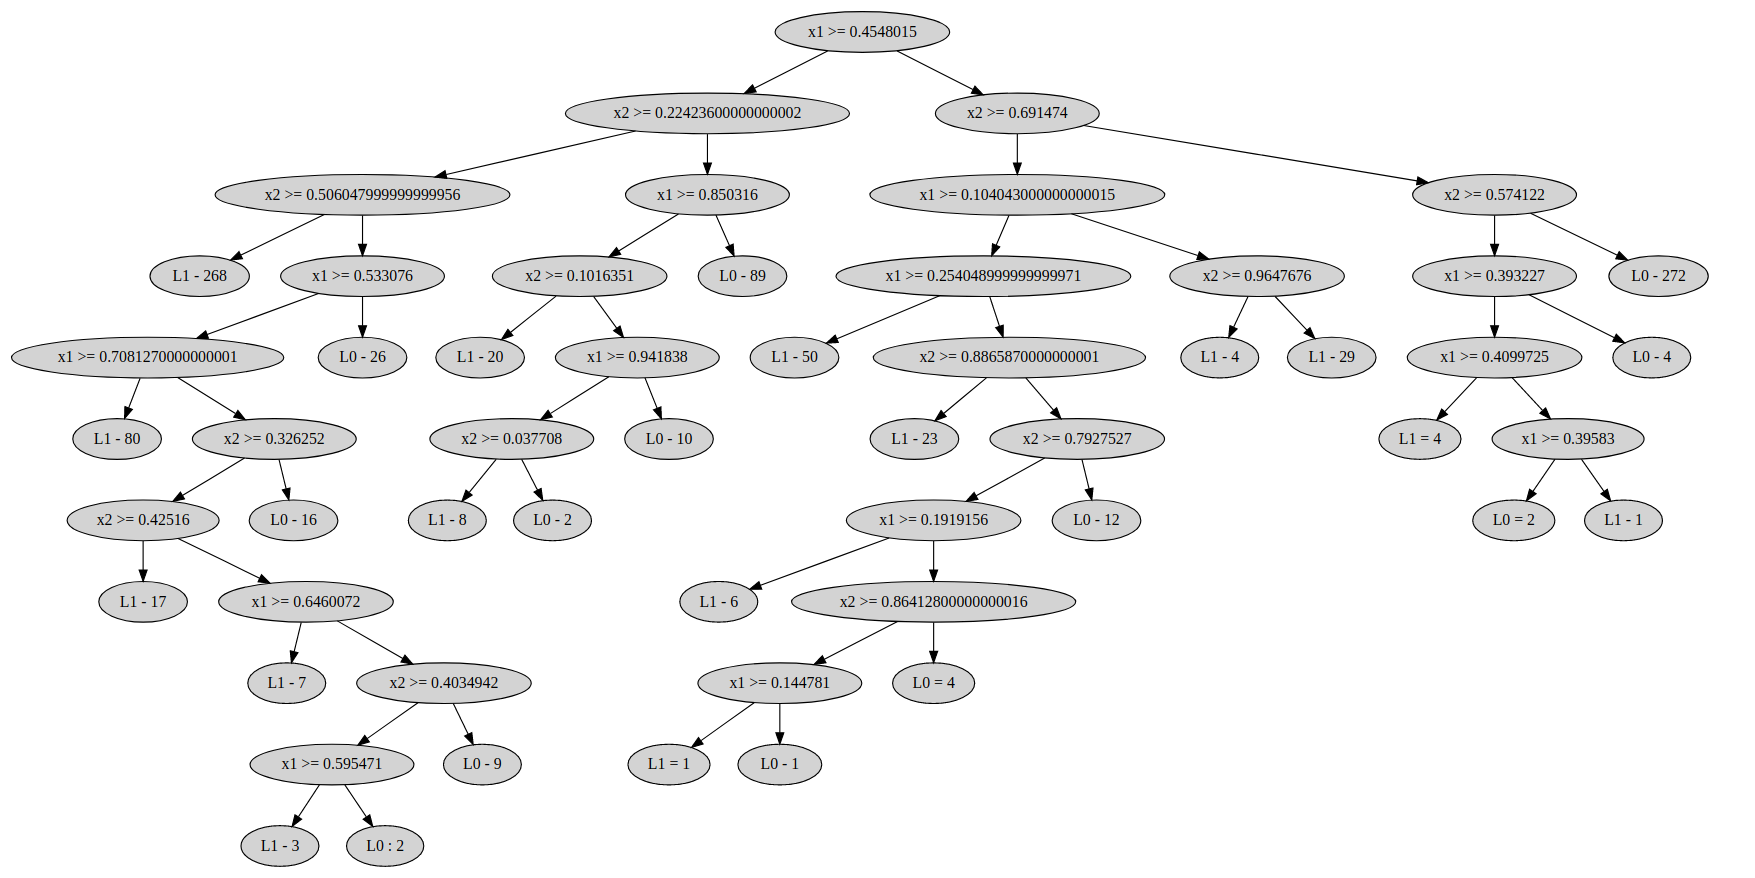
\includegraphics[width=1.1\textwidth]{D2_tree.png}
  		\captionsetup{labelformat=empty}
  		\caption{}
  		\label{fig:my_label}
  	\end{figure}
  	
  \end{soln}
  \item Try to interpret your D2 decision tree.
  
	\begin{soln}
		Quite evidently, the decision tree for D2.txt is much more complex, as seen from the large number of attribute decisions being made at each level. Since, the decision boundaries are parallel to the axes, such a large number of decision points suggests two possibilities: firstly, complicated island like enclosures of datapoints, or secondly, a sloped linear decision boundary in the x-space. Put simply, we note, that the first split conditions on x1 and successive decision boundaries keep partitioning the top-left and bottom right quadrant of the space. This could suggest a negatively sloped decision boundary. The tree's decision points can be interpreted as a depthwise series of decisions being made, such that it can fit the training data.
	\end{soln}
  \end{itemize}

\item (Hypothesis space)  [10 pts] For D1.txt and D2.txt, do the following separately:
  \begin{itemize}
  \item Produce a scatter plot of the data set.
  
  
    \begin{soln}
	The scatter plot for D1.txt
	\begin{figure}[H]
		\centering
		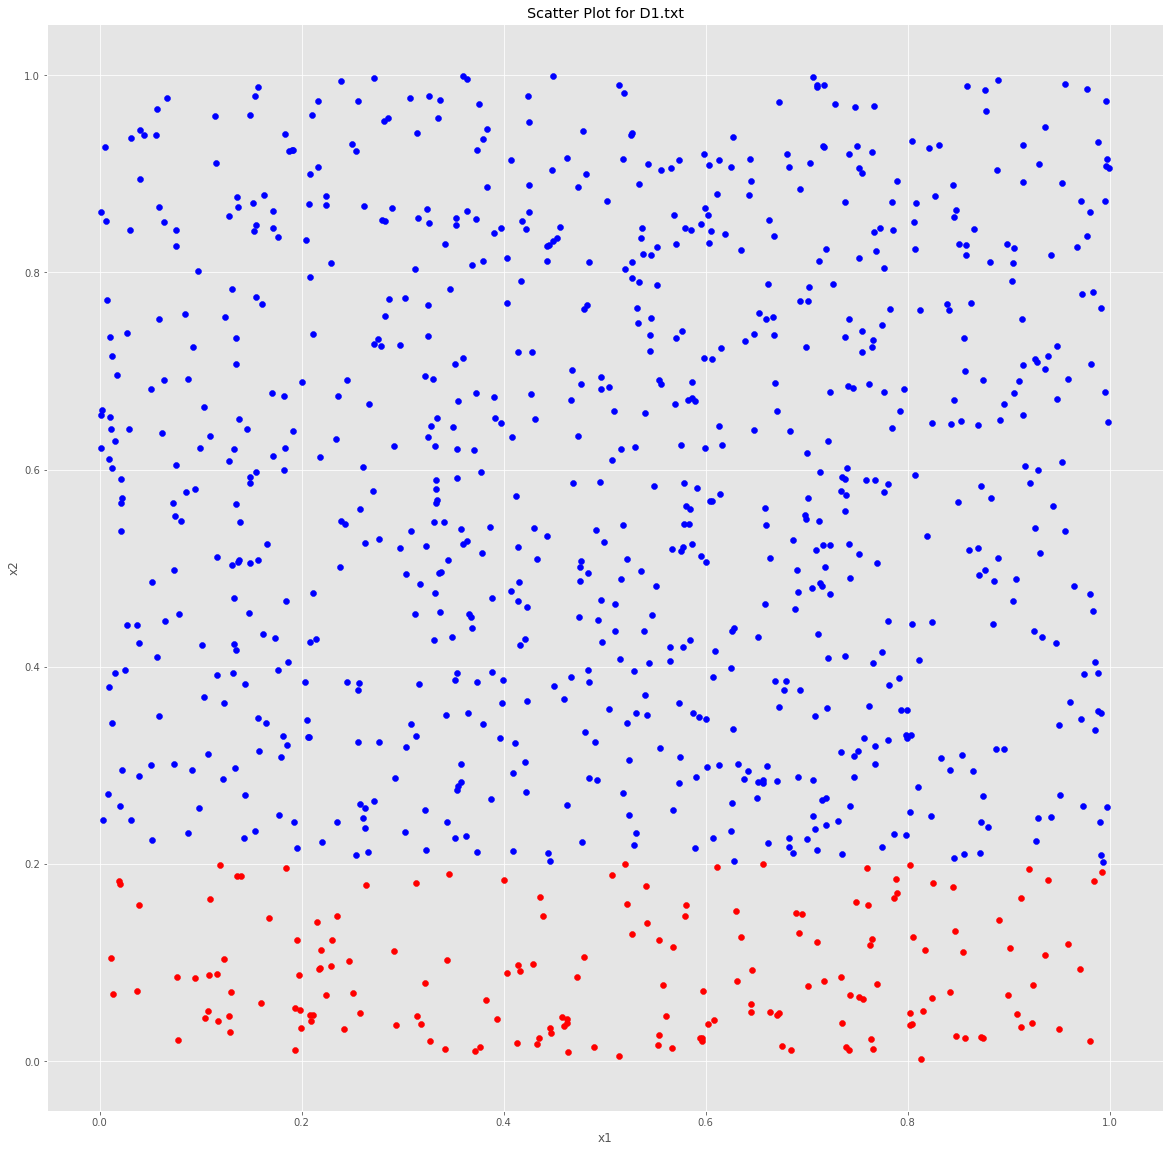
\includegraphics[width=1.1\textwidth]{D1_scatter.png}
		\captionsetup{labelformat=empty}
		\caption{}
		\label{fig:my_label}
	\end{figure}
	\vspace{0.5cm}
	The scatter plot for D2.txt
	
	\begin{figure}[H]
		\centering
		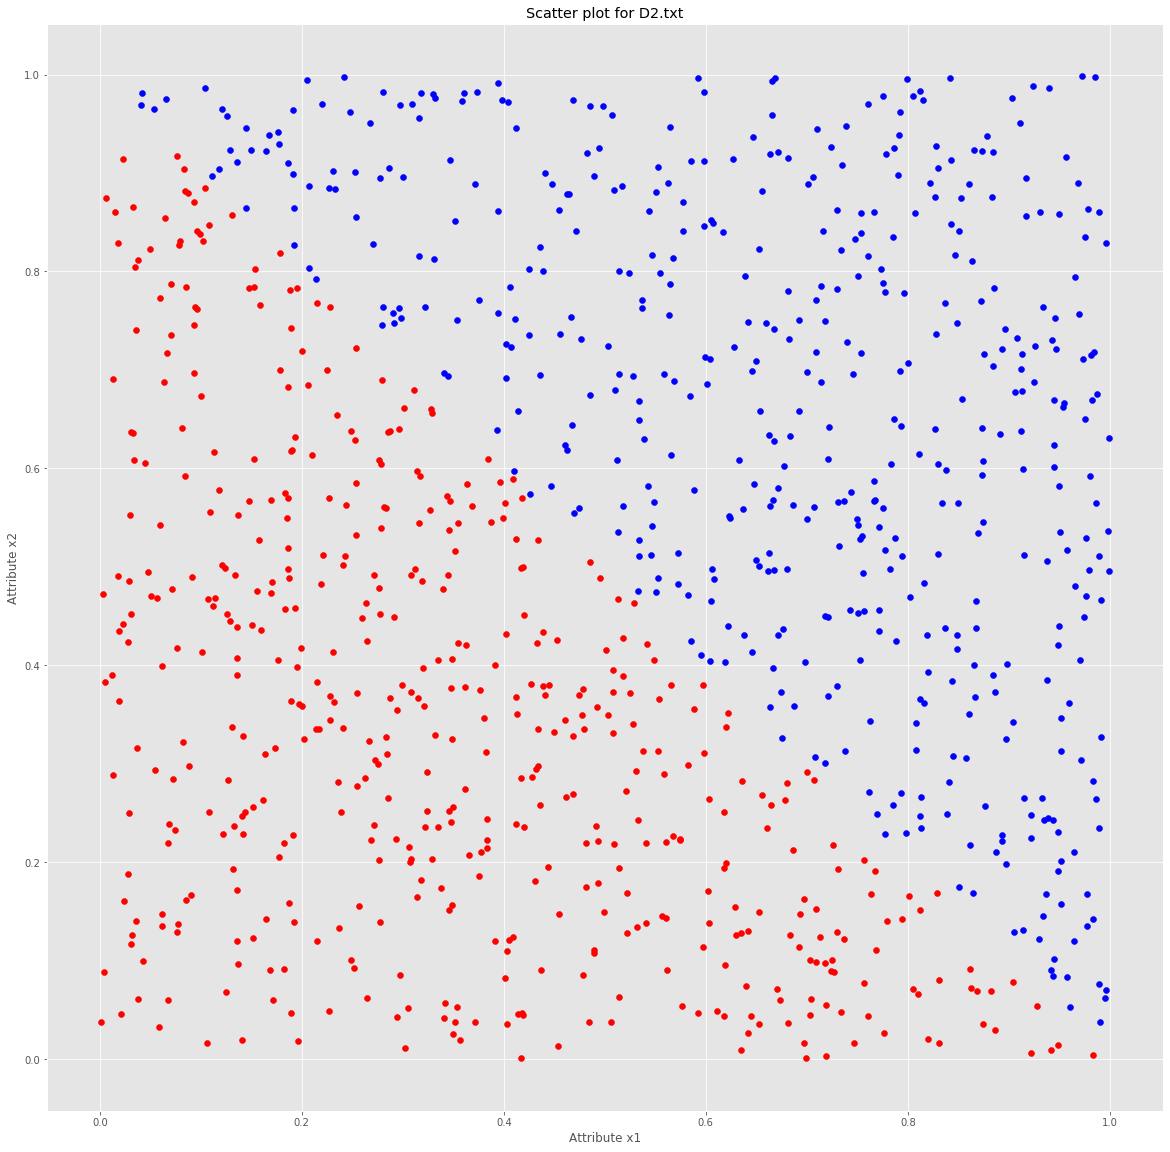
\includegraphics[width=1.1\textwidth]{D2_scatter.png}
		\captionsetup{labelformat=empty}
		\caption{}
		\label{fig:my_label}
	\end{figure}
	
	
\end{soln}

  \item Visualize your decision tree's decision boundary (or decision region, or some other ways to clearly visualize how your decision tree will make decisions in the feature space).
  
    \begin{soln}
  	The scatter plot for D1.txt with Decision Boundary
  	  	\begin{figure}[H]
  		\centering
  		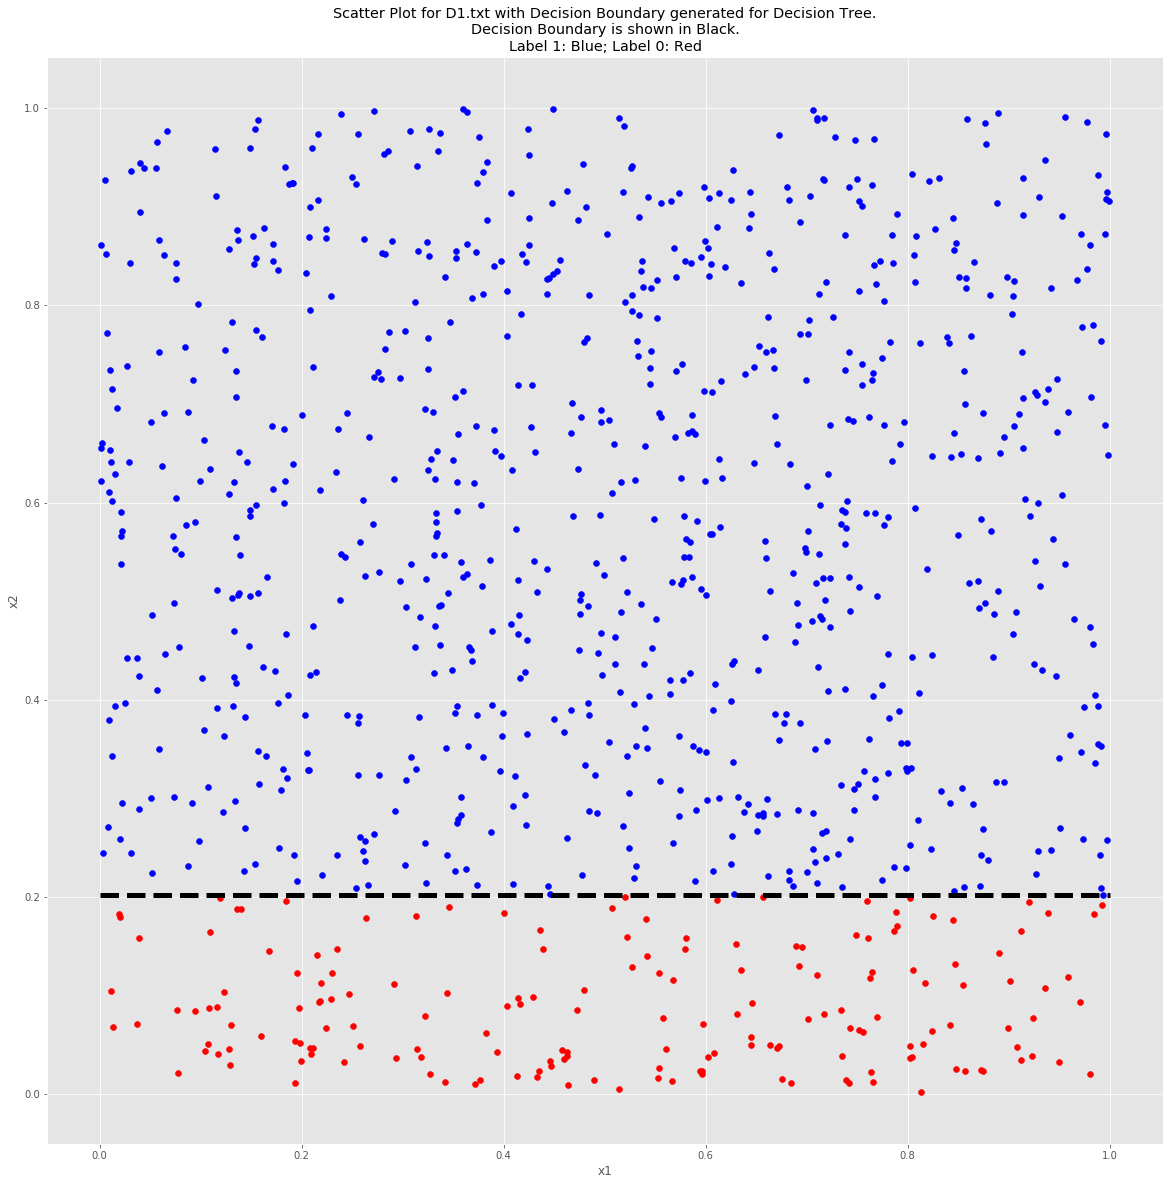
\includegraphics[width=1.1\textwidth]{D1_DecisionBoundary.png}
  		\captionsetup{labelformat=empty}
  		\caption{}
  		\label{fig:my_label}
  	\end{figure}
  	
  	The scatter plot for D2.txt with Decision Boundary
  	
  	  	\begin{figure}[H]
  		\centering
  		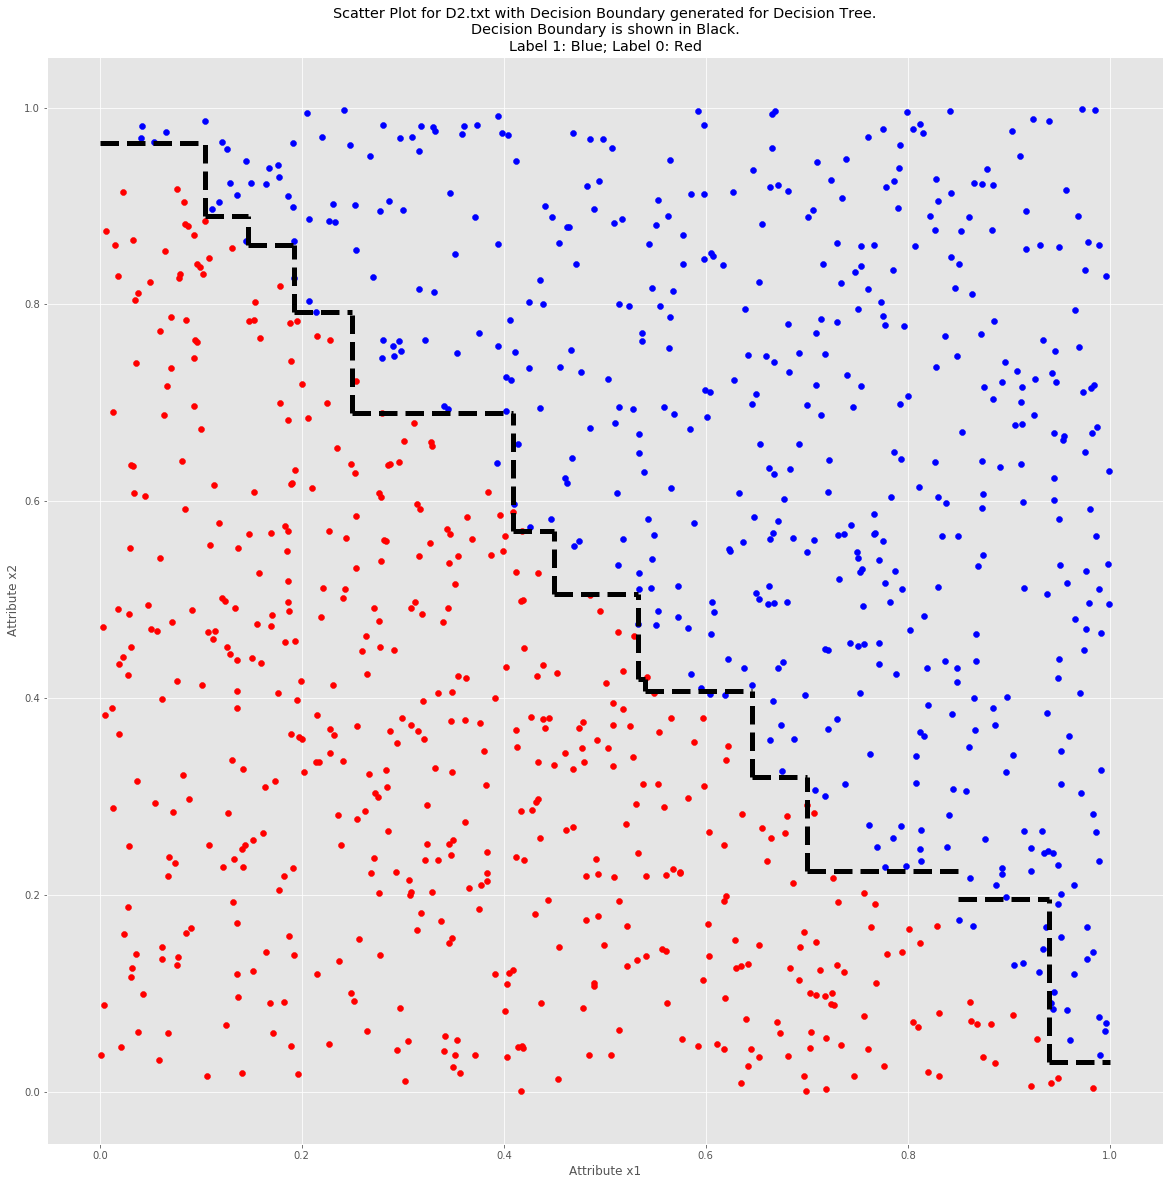
\includegraphics[width=1.1\textwidth]{D2_DecisionBoundary.png}
  		\captionsetup{labelformat=empty}
  		\caption{}
  		\label{fig:my_label}
  	\end{figure}
  	
  	
  \end{soln}
  \end{itemize}


Then discuss why the size of your decision trees on D1 and D2 differ.  Relate this to the hypothesis space of our decision tree algorithm. 

\begin{soln}
	As discussed and hypothesized in Question 6, the decision boundary for D1 essentially turned out to be a straight line parallel to the x1 axis. Moreover, due to the large number of decision splits concentrated in the top-left and bottom-right quadrant of the space, we notice a negatively sloped decision boundary for D2.txt. Evidently, the decision tree boundary is trying to approximate the $y = -x$ line in D2, and that's approximately how the training data seems to be separated as well. (Note: The decision tree boundary has been crudely plotted using decision pivot points, and thus, can include some noise). Since, decision trees can plot axes-parallel decision boundaries, it becomes difficult to model a decision boundary that looks like $y = -x$. Thus, small sections of the decision boundary is drawn, with a general tendency of $x2$ split magnitudes to go down as $x1$ increases. 
\end{soln}

\item (Learning curve)  [20 pts] We provide a data set Dbig.txt with 10000 labeled items.  Caution: Dbig.txt is sorted.
  \begin{itemize}
  \item You will randomly split Dbig.txt into a candidate training set of 8192 items and a test set (the rest).  Do this by generating a random permutation, and split at 8192.
  \item Generate a sequence of five nested training sets $D_{32} \subset D_{128} \subset D_{512} \subset D_{2048} \subset D_{8192}$ from the candidate training set.  The subscript $n$ in $D_n$ denotes training set size.  The easiest way is to take the first $n$ items from the (same) permutation above.  This sequence simulates the real world situation where you obtain more and more training data.
  \item For each $D_n$ above, train a decision tree.  Measure its test set error $err_n$.  Show three things in your answer: (1) List $n$, number of nodes in that tree, $err_n$. (2) Plot $n$ vs. $err_n$.  This is known as a learning curve (a single plot). (3) Visualize your decision trees' decision boundary (five plots).
  \end{itemize}

\end{enumerate}

\begin{soln}
	\begin{itemize}
		\item The number of nodes in each tree is summarized as follows: 	
	\end{itemize}
	\begin{center}
	\begin{tabular}{ c c }
		training-size &  nodes \\
		32 &  4\\ 
		128 & 7 \\
		512 & 17 \\
		2048 & 49  \\
		8192 & 118
	\end{tabular}
\end{center}

\begin{itemize}
	\item The learning curve is as follows. Error reduces as we increase number of training points.
\end{itemize}

\begin{figure}[H]
	\centering
	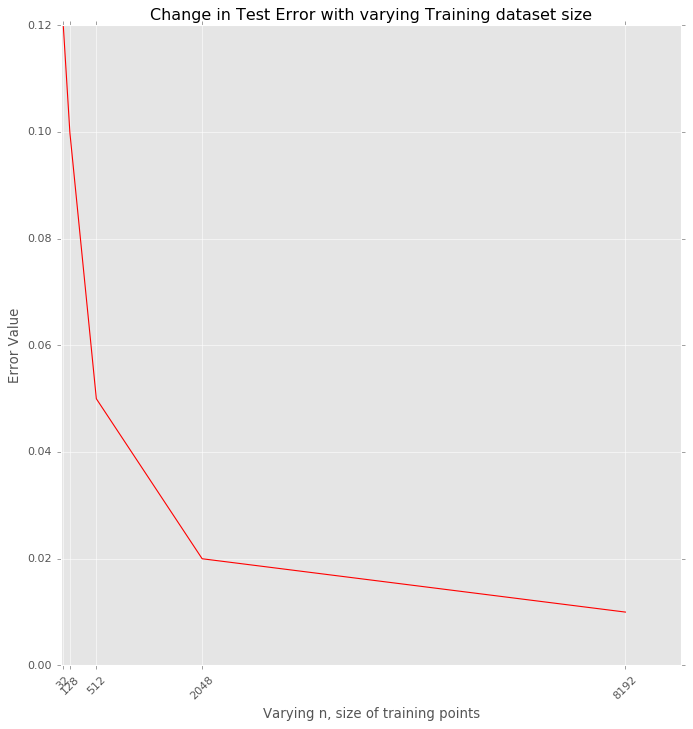
\includegraphics[width=0.8\textwidth]{err_n.png}
	\captionsetup{labelformat=empty}
	\caption{}
	\label{fig:my_label}
\end{figure}


\begin{itemize}
	\item The decision boundary figures are attached as follows
	\item Note: In each of the figure, the decision boundary is at the edge of the two differently colored regions. So, for instance, a decision boundary will be formed along the edge the red and blue patches are meeting.

\end{itemize}

N = 32

\begin{figure}[H]
	\centering
	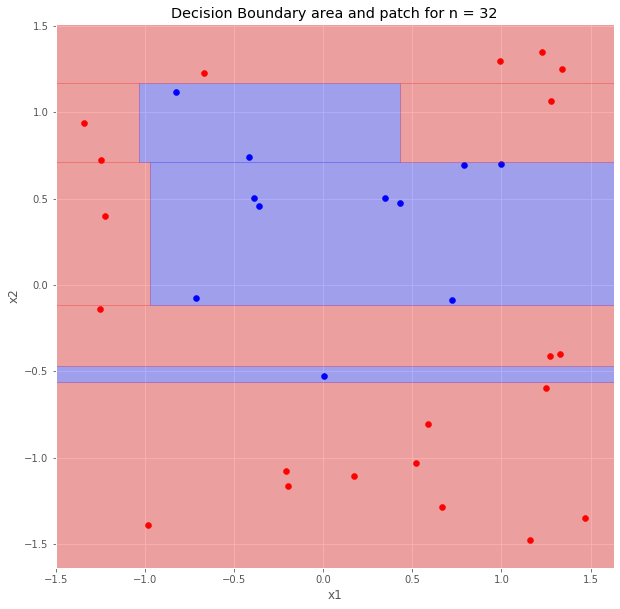
\includegraphics[width=0.6\textwidth]{n_32.png}
	\captionsetup{labelformat=empty}
	\caption{}
	\label{fig:my_label}
\end{figure}

N = 128

\begin{figure}[H]
	\centering
	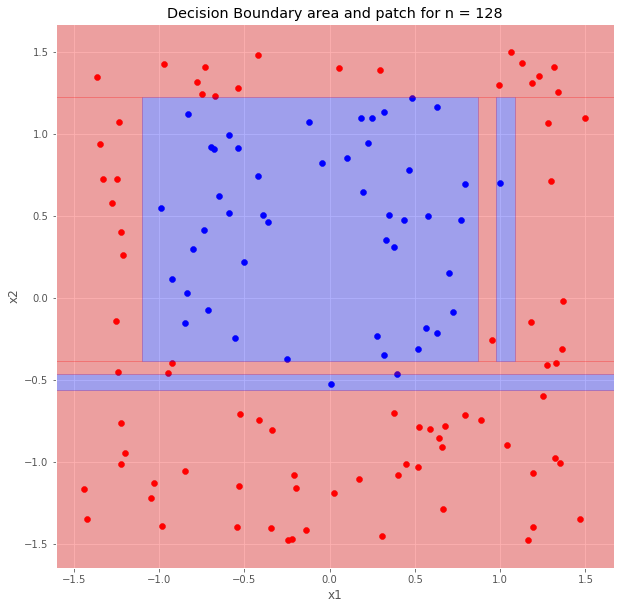
\includegraphics[width=0.6\textwidth]{n_128.png}
	\captionsetup{labelformat=empty}
	\caption{}
	\label{fig:my_label}
\end{figure}

N = 512

\begin{figure}[H]
	\centering
	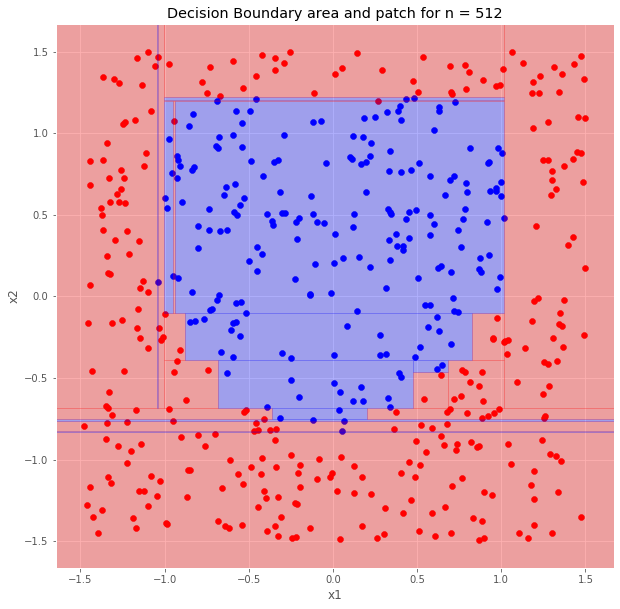
\includegraphics[width=0.6\textwidth]{n_512.png}
	\captionsetup{labelformat=empty}
	\caption{}
	\label{fig:my_label}
\end{figure}

N = 2048

\begin{figure}[H]
	\centering
	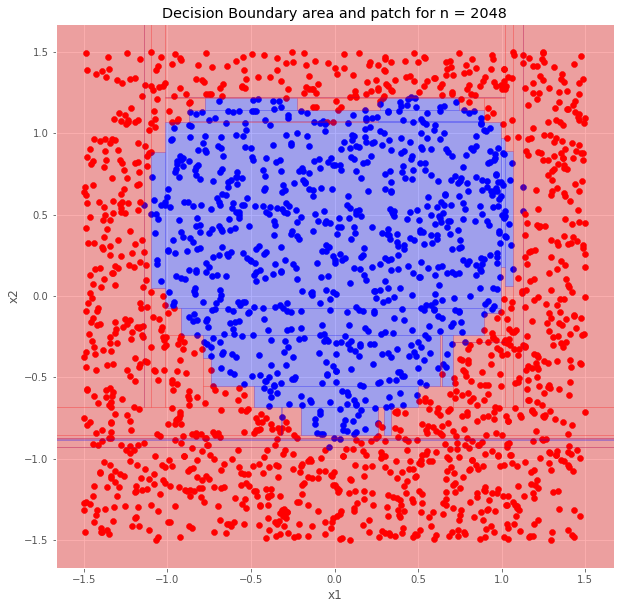
\includegraphics[width=0.6\textwidth]{n_2048.png}
	\captionsetup{labelformat=empty}
	\caption{}
	\label{fig:my_label}
\end{figure}


N = 8192

\begin{figure}[H]
	\centering
	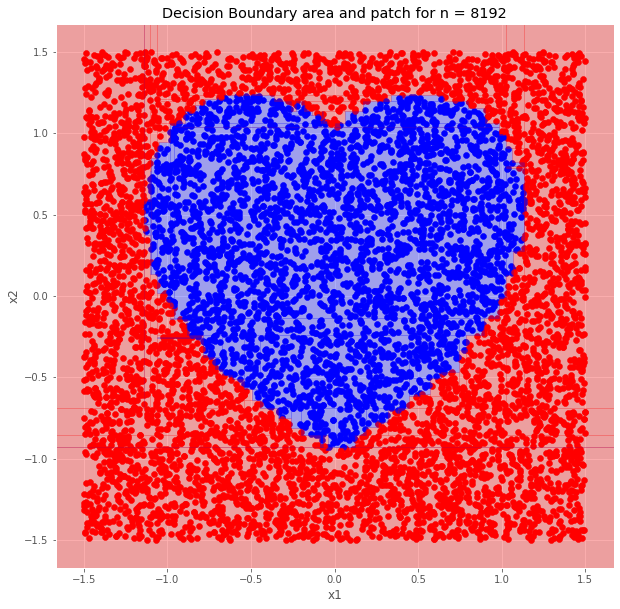
\includegraphics[width=0.6\textwidth]{n_8192.png}
	\captionsetup{labelformat=empty}
	\caption{}
	\label{fig:my_label}
\end{figure}
\end{soln}

\section{Weka [10 pts]}
Learn to use Weka \url{https://www.cs.waikato.ac.nz/~ml/weka/index.html}.
Convert appropriate data files into ARFF format.
Use trees/J48 as the classifier and default settings.
Produce five Weka trees for $D_{32}, D_{128} \ldots D_{8192}$.  
Show two things in your answer: (1) List $n$, number of nodes in that tree, $err_n$. (2) Plot $n$ vs. $err_n$.





Plot of error value across different training sizes for weka trained decision tree is as follows:


\begin{soln}
	
	
\begin{itemize}
	\item The number of nodes in each tree is summarized as follows: 	
\end{itemize}
\begin{center}
	\begin{tabular}{ c c }
		training-size &  nodes \\
		32 &  4\\ 
		128 & 4 \\
		512 & 11 \\
		2048 & 25  \\
		8192 & 77
	\end{tabular}
\end{center}

\begin{itemize}
	\item The learning curve is as follows. Error reduces as we increase number of training points.
\end{itemize}

\begin{figure}[H]
	\centering
	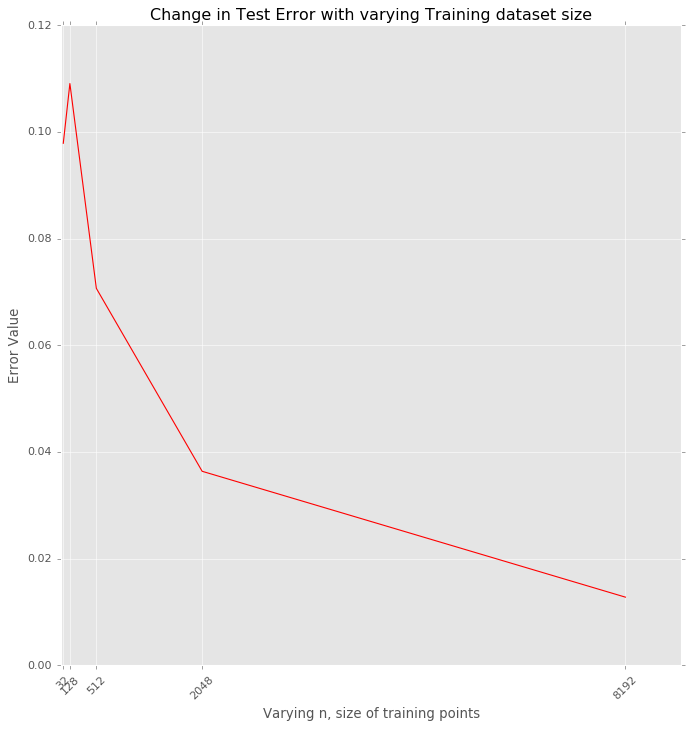
\includegraphics[width=0.8\textwidth]{err_n_weka.png}
	\captionsetup{labelformat=empty}
	\caption{}
	\label{fig:my_label}
\end{figure}

PS: The trees associated with each training set has also been attached below for reference.
	
\begin{itemize}
	\item \textbf{n = 32, Number of nodes = 4, Leaves = 5}
\end{itemize}
Tree:


\begin{lstlisting}

attribute_1 <= -0.599203: 1.0 (10.0)
attribute_1 > -0.599203
|   attribute_0 <= 0.996712
|   |   attribute_0 <= -1.223955: 1.0 (4.0)
|   |   attribute_0 > -1.223955
|   |   |   attribute_1 <= 1.117817: 0.0 (11.0)
|   |   |   attribute_1 > 1.117817: 1.0 (2.0)
|   attribute_0 > 0.996712: 1.0 (5.0)

Number of Leaves  : 	5

Size of the tree : 	9


\end{lstlisting}

\vspace{1cm}



\begin{itemize}
	\item \textbf{n = 128, Number of nodes = 4, Leaves = 5}
\end{itemize}
Tree:


\begin{lstlisting}


attribute_1 <= -0.599203: 1.0 (43.0)
attribute_1 > -0.599203
|   attribute_1 <= 1.217759
|   |   attribute_0 <= -0.924705: 1.0 (12.0/1.0)
|   |   attribute_0 > -0.924705
|   |   |   attribute_0 <= 0.7934: 0.0 (46.0)
|   |   |   attribute_0 > 0.7934: 1.0 (10.0/1.0)
|   attribute_1 > 1.217759: 1.0 (17.0)

Number of Leaves  : 	5

Size of the tree : 	9



\end{lstlisting}

\vspace{1cm}


\begin{itemize}
	\item \textbf{n = 512, Number of nodes = 11, Leaves = 12}
\end{itemize}
Tree:


\begin{lstlisting}


attribute_1 <= -0.76503: 1.0 (131.0/1.0)
attribute_1 > -0.76503
|   attribute_0 <= 1.013339
|   |   attribute_0 <= -1.008838: 1.0 (58.0/1.0)
|   |   attribute_0 > -1.008838
|   |   |   attribute_1 <= 1.217759
|   |   |   |   attribute_1 <= -0.251567
|   |   |   |   |   attribute_0 <= 0.709315
|   |   |   |   |   |   attribute_0 <= -0.715157: 1.0 (6.0)
|   |   |   |   |   |   attribute_0 > -0.715157
|   |   |   |   |   |   |   attribute_1 <= -0.686172
|   |   |   |   |   |   |   |   attribute_1 <= -0.753451: 0.0 (2.0)
|   |   |   |   |   |   |   |   attribute_1 > -0.753451: 1.0 (8.0/2.0)
|   |   |   |   |   |   |   attribute_1 > -0.686172
|   |   |   |   |   |   |   |   attribute_0 <= 0.525442: 0.0 (22.0)
|   |   |   |   |   |   |   |   attribute_0 > 0.525442
|   |   |   |   |   |   |   |   |   attribute_1 <= -0.46243: 1.0 (2.0)
|   |   |   |   |   |   |   |   |   attribute_1 > -0.46243: 0.0 (3.0)
|   |   |   |   |   attribute_0 > 0.709315: 1.0 (15.0)
|   |   |   |   attribute_1 > -0.251567: 0.0 (180.0/4.0)
|   |   |   attribute_1 > 1.217759: 1.0 (31.0)
|   attribute_0 > 1.013339: 1.0 (54.0)

Number of Leaves  : 	12

Size of the tree : 	23


\end{lstlisting}

\vspace{1cm}



\begin{itemize}
	\item \textbf{n = 2048, Number of nodes = 25, Leaves = 26}
\end{itemize}
Tree:


\begin{lstlisting}


attribute_1 <= -0.701439
|   attribute_1 <= -0.930001: 1.0 (424.0)
|   attribute_1 > -0.930001
|   |   attribute_0 <= 0.260772
|   |   |   attribute_0 <= -0.171836: 1.0 (71.0/1.0)
|   |   |   attribute_0 > -0.171836
|   |   |   |   attribute_1 <= -0.857016
|   |   |   |   |   attribute_0 <= 0.078937: 0.0 (3.0)
|   |   |   |   |   attribute_0 > 0.078937: 1.0 (5.0)
|   |   |   |   attribute_1 > -0.857016: 0.0 (17.0)
|   |   attribute_0 > 0.260772: 1.0 (73.0)
attribute_1 > -0.701439
|   attribute_0 <= 1.068273
|   |   attribute_0 <= -1.097661: 1.0 (183.0/1.0)
|   |   attribute_0 > -1.097661
|   |   |   attribute_1 <= 1.219689
|   |   |   |   attribute_1 <= -0.097383
|   |   |   |   |   attribute_0 <= 0.71112
|   |   |   |   |   |   attribute_0 <= -0.871352: 1.0 (31.0)
|   |   |   |   |   |   attribute_0 > -0.871352
|   |   |   |   |   |   |   attribute_1 <= -0.552516
|   |   |   |   |   |   |   |   attribute_0 <= -0.470132: 1.0 (10.0)
|   |   |   |   |   |   |   |   attribute_0 > -0.470132
|   |   |   |   |   |   |   |   |   attribute_0 <= 0.498051: 0.0 (29.0)
|   |   |   |   |   |   |   |   |   attribute_0 > 0.498051: 1.0 (8.0)
|   |   |   |   |   |   |   attribute_1 > -0.552516
|   |   |   |   |   |   |   |   attribute_0 <= -0.739759
|   |   |   |   |   |   |   |   |   attribute_1 <= -0.322227: 1.0 (3.0)
|   |   |   |   |   |   |   |   |   attribute_1 > -0.322227: 0.0 (11.0)
|   |   |   |   |   |   |   |   attribute_0 > -0.739759: 0.0 (128.0/1.0)
|   |   |   |   |   attribute_0 > 0.71112
|   |   |   |   |   |   attribute_1 <= -0.281487: 1.0 (38.0)
|   |   |   |   |   |   attribute_1 > -0.281487
|   |   |   |   |   |   |   attribute_0 <= 0.893663: 0.0 (5.0/1.0)
|   |   |   |   |   |   |   attribute_0 > 0.893663: 1.0 (13.0)
|   |   |   |   attribute_1 > -0.097383
|   |   |   |   |   attribute_1 <= 1.037938
|   |   |   |   |   |   attribute_1 <= 0.001005
|   |   |   |   |   |   |   attribute_0 <= 0.982898
|   |   |   |   |   |   |   |   attribute_0 <= -0.963055: 1.0 (4.0/1.0)
|   |   |   |   |   |   |   |   attribute_0 > -0.963055: 0.0 (49.0)
|   |   |   |   |   |   |   attribute_0 > 0.982898: 1.0 (3.0)
|   |   |   |   |   |   attribute_1 > 0.001005: 0.0 (494.0/1.0)
|   |   |   |   |   attribute_1 > 1.037938
|   |   |   |   |   |   attribute_0 <= -0.903972: 1.0 (8.0)
|   |   |   |   |   |   attribute_0 > -0.903972
|   |   |   |   |   |   |   attribute_0 <= 0.894953: 0.0 (81.0/14.0)
|   |   |   |   |   |   |   attribute_0 > 0.894953: 1.0 (5.0)
|   |   |   attribute_1 > 1.219689: 1.0 (139.0)
|   attribute_0 > 1.068273: 1.0 (213.0/2.0)

Number of Leaves  : 	26

Size of the tree : 	51


\end{lstlisting}

\vspace{1cm}

\begin{itemize}
	\item \textbf{n = 8192, Number of nodes = 77, Leaves = 78}
\end{itemize}
Tree:


\begin{lstlisting}

attribute_1 <= -0.69923
|   attribute_1 <= -0.926919: 1.0 (1620.0)
|   attribute_1 > -0.926919
|   |   attribute_0 <= -0.336447: 1.0 (254.0)
|   |   attribute_0 > -0.336447
|   |   |   attribute_0 <= 0.321717
|   |   |   |   attribute_1 <= -0.78646
|   |   |   |   |   attribute_0 <= -0.198645: 1.0 (16.0)
|   |   |   |   |   attribute_0 > -0.198645
|   |   |   |   |   |   attribute_0 <= 0.143166
|   |   |   |   |   |   |   attribute_1 <= -0.87181
|   |   |   |   |   |   |   |   attribute_0 <= -0.088258: 1.0 (3.0)
|   |   |   |   |   |   |   |   attribute_0 > -0.088258: 0.0 (13.0/2.0)
|   |   |   |   |   |   |   attribute_1 > -0.87181: 0.0 (27.0)
|   |   |   |   |   |   attribute_0 > 0.143166: 1.0 (19.0/1.0)
|   |   |   |   attribute_1 > -0.78646
|   |   |   |   |   attribute_0 <= -0.248678
|   |   |   |   |   |   attribute_1 <= -0.74829: 1.0 (3.0)
|   |   |   |   |   |   attribute_1 > -0.74829: 0.0 (5.0)
|   |   |   |   |   attribute_0 > -0.248678: 0.0 (36.0)
|   |   |   attribute_0 > 0.321717: 1.0 (249.0)
attribute_1 > -0.69923
|   attribute_1 <= 1.231492
|   |   attribute_0 <= 1.067352
|   |   |   attribute_0 <= -1.105675
|   |   |   |   attribute_0 <= -1.13935: 1.0 (649.0)
|   |   |   |   attribute_0 > -1.13935
|   |   |   |   |   attribute_1 <= 0.372775: 1.0 (22.0)
|   |   |   |   |   attribute_1 > 0.372775
|   |   |   |   |   |   attribute_1 <= 0.585209: 0.0 (6.0/1.0)
|   |   |   |   |   |   attribute_1 > 0.585209: 1.0 (11.0)
|   |   |   attribute_0 > -1.105675
|   |   |   |   attribute_1 <= -0.203086
|   |   |   |   |   attribute_0 <= -0.765869
|   |   |   |   |   |   attribute_0 <= -0.857225: 1.0 (119.0)
|   |   |   |   |   |   attribute_0 > -0.857225
|   |   |   |   |   |   |   attribute_1 <= -0.286624: 1.0 (38.0/1.0)
|   |   |   |   |   |   |   attribute_1 > -0.286624: 0.0 (8.0/1.0)
|   |   |   |   |   attribute_0 > -0.765869
|   |   |   |   |   |   attribute_0 <= 0.68416
|   |   |   |   |   |   |   attribute_0 <= -0.528159
|   |   |   |   |   |   |   |   attribute_1 <= -0.487421: 1.0 (47.0/2.0)
|   |   |   |   |   |   |   |   attribute_1 > -0.487421
|   |   |   |   |   |   |   |   |   attribute_1 <= -0.402784
|   |   |   |   |   |   |   |   |   |   attribute_0 <= -0.697592: 1.0 (8.0/1.0)
|   |   |   |   |   |   |   |   |   |   attribute_0 > -0.697592: 0.0 (9.0)
|   |   |   |   |   |   |   |   |   attribute_1 > -0.402784: 0.0 (40.0)
|   |   |   |   |   |   |   attribute_0 > -0.528159
|   |   |   |   |   |   |   |   attribute_0 <= 0.447026
|   |   |   |   |   |   |   |   |   attribute_0 <= -0.444559
|   |   |   |   |   |   |   |   |   |   attribute_1 <= -0.642578: 1.0 (4.0)
|   |   |   |   |   |   |   |   |   |   attribute_1 > -0.642578: 0.0 (32.0)
|   |   |   |   |   |   |   |   |   attribute_0 > -0.444559: 0.0 (401.0)
|   |   |   |   |   |   |   |   attribute_0 > 0.447026
|   |   |   |   |   |   |   |   |   attribute_1 <= -0.477942
|   |   |   |   |   |   |   |   |   |   attribute_1 <= -0.614785: 1.0 (17.0)
|   |   |   |   |   |   |   |   |   |   attribute_1 > -0.614785
|   |   |   |   |   |   |   |   |   |   |   attribute_0 <= 0.612795: 0.0 (17.0/2.0)
|   |   |   |   |   |   |   |   |   |   |   attribute_0 > 0.612795: 1.0 (11.0)
|   |   |   |   |   |   |   |   |   attribute_1 > -0.477942: 0.0 (69.0)
|   |   |   |   |   |   attribute_0 > 0.68416
|   |   |   |   |   |   |   attribute_0 <= 0.788976
|   |   |   |   |   |   |   |   attribute_1 <= -0.384086: 1.0 (32.0)
|   |   |   |   |   |   |   |   attribute_1 > -0.384086: 0.0 (16.0/1.0)
|   |   |   |   |   |   |   attribute_0 > 0.788976: 1.0 (128.0/1.0)
|   |   |   |   attribute_1 > -0.203086
|   |   |   |   |   attribute_1 <= 1.033115
|   |   |   |   |   |   attribute_0 <= -0.963055
|   |   |   |   |   |   |   attribute_1 <= 0.06749
|   |   |   |   |   |   |   |   attribute_0 <= -0.993641: 1.0 (20.0)
|   |   |   |   |   |   |   |   attribute_0 > -0.993641
|   |   |   |   |   |   |   |   |   attribute_1 <= -0.055302: 1.0 (5.0)
|   |   |   |   |   |   |   |   |   attribute_1 > -0.055302: 0.0 (6.0/1.0)
|   |   |   |   |   |   |   attribute_1 > 0.06749
|   |   |   |   |   |   |   |   attribute_1 <= 0.812138: 0.0 (97.0/2.0)
|   |   |   |   |   |   |   |   attribute_1 > 0.812138
|   |   |   |   |   |   |   |   |   attribute_0 <= -1.069359: 1.0 (3.0)
|   |   |   |   |   |   |   |   |   attribute_0 > -1.069359: 0.0 (13.0/2.0)
|   |   |   |   |   |   attribute_0 > -0.963055
|   |   |   |   |   |   |   attribute_0 <= 0.984975
|   |   |   |   |   |   |   |   attribute_1 <= -0.133802
|   |   |   |   |   |   |   |   |   attribute_0 <= -0.859894
|   |   |   |   |   |   |   |   |   |   attribute_0 <= -0.900757: 1.0 (3.0)
|   |   |   |   |   |   |   |   |   |   attribute_0 > -0.900757: 0.0 (3.0)
|   |   |   |   |   |   |   |   |   attribute_0 > -0.859894
|   |   |   |   |   |   |   |   |   |   attribute_0 <= 0.866694: 0.0 (92.0)
|   |   |   |   |   |   |   |   |   |   attribute_0 > 0.866694
|   |   |   |   |   |   |   |   |   |   |   attribute_0 <= 0.900121: 0.0 (2.0)
|   |   |   |   |   |   |   |   |   |   |   attribute_0 > 0.900121: 1.0 (3.0)
|   |   |   |   |   |   |   |   attribute_1 > -0.133802: 0.0 (2019.0)
|   |   |   |   |   |   |   attribute_0 > 0.984975
|   |   |   |   |   |   |   |   attribute_1 <= 0.076669
|   |   |   |   |   |   |   |   |   attribute_1 <= -0.005703: 1.0 (18.0)
|   |   |   |   |   |   |   |   |   attribute_1 > -0.005703
|   |   |   |   |   |   |   |   |   |   attribute_0 <= 1.012294: 0.0 (2.0)
|   |   |   |   |   |   |   |   |   |   attribute_0 > 1.012294: 1.0 (3.0)
|   |   |   |   |   |   |   |   attribute_1 > 0.076669
|   |   |   |   |   |   |   |   |   attribute_1 <= 0.933382: 0.0 (58.0)
|   |   |   |   |   |   |   |   |   attribute_1 > 0.933382
|   |   |   |   |   |   |   |   |   |   attribute_0 <= 1.013339
|   |   |   |   |   |   |   |   |   |   |   attribute_1 <= 0.998045: 0.0 (4.0)
|   |   |   |   |   |   |   |   |   |   |   attribute_1 > 0.998045: 1.0 (2.0)
|   |   |   |   |   |   |   |   |   |   attribute_0 > 1.013339: 1.0 (4.0)
|   |   |   |   |   attribute_1 > 1.033115
|   |   |   |   |   |   attribute_0 <= -0.898152
|   |   |   |   |   |   |   attribute_1 <= 1.062305
|   |   |   |   |   |   |   |   attribute_0 <= -0.986041: 1.0 (4.0)
|   |   |   |   |   |   |   |   attribute_0 > -0.986041: 0.0 (3.0)
|   |   |   |   |   |   |   attribute_1 > 1.062305: 1.0 (35.0)
|   |   |   |   |   |   attribute_0 > -0.898152
|   |   |   |   |   |   |   attribute_0 <= 0.900815
|   |   |   |   |   |   |   |   attribute_1 <= 1.188319
|   |   |   |   |   |   |   |   |   attribute_0 <= 0.139429
|   |   |   |   |   |   |   |   |   |   attribute_0 <= -0.161295
|   |   |   |   |   |   |   |   |   |   |   attribute_1 <= 1.143059: 0.0 (71.0)
|   |   |   |   |   |   |   |   |   |   |   attribute_1 > 1.143059
|   |   |   |   |   |   |   |   |   |   |   |   attribute_0 <= -0.819483: 1.0 (4.0)
|   |   |   |   |   |   |   |   |   |   |   |   attribute_0 > -0.819483
|   |   |   |   |   |   |   |   |   |   |   |   |   attribute_0 <= -0.250788: 0.0 (28.0)
|   |   |   |   |   |   |   |   |   |   |   |   |   attribute_0 > -0.250788
|   |   |   |   |   |   |   |   |   |   |   |   |   |   attribute_1 <= 1.175016: 0.0 (2.0)
|   |   |   |   |   |   |   |   |   |   |   |   |   |   attribute_1 > 1.175016: 1.0 (2.0)
|   |   |   |   |   |   |   |   |   |   attribute_0 > -0.161295
|   |   |   |   |   |   |   |   |   |   |   attribute_1 <= 1.11299
|   |   |   |   |   |   |   |   |   |   |   |   attribute_0 <= 0.024432
|   |   |   |   |   |   |   |   |   |   |   |   |   attribute_0 <= -0.052428: 0.0 (9.0/1.0)
|   |   |   |   |   |   |   |   |   |   |   |   |   attribute_0 > -0.052428: 1.0 (10.0)
|   |   |   |   |   |   |   |   |   |   |   |   attribute_0 > 0.024432: 0.0 (5.0)
|   |   |   |   |   |   |   |   |   |   |   attribute_1 > 1.11299: 1.0 (16.0)
|   |   |   |   |   |   |   |   |   attribute_0 > 0.139429
|   |   |   |   |   |   |   |   |   |   attribute_1 <= 1.172419: 0.0 (98.0)
|   |   |   |   |   |   |   |   |   |   attribute_1 > 1.172419
|   |   |   |   |   |   |   |   |   |   |   attribute_0 <= 0.786886: 0.0 (9.0)
|   |   |   |   |   |   |   |   |   |   |   attribute_0 > 0.786886: 1.0 (2.0)
|   |   |   |   |   |   |   |   attribute_1 > 1.188319
|   |   |   |   |   |   |   |   |   attribute_0 <= -0.313669
|   |   |   |   |   |   |   |   |   |   attribute_0 <= -0.663159: 1.0 (11.0/2.0)
|   |   |   |   |   |   |   |   |   |   attribute_0 > -0.663159: 0.0 (18.0)
|   |   |   |   |   |   |   |   |   attribute_0 > -0.313669
|   |   |   |   |   |   |   |   |   |   attribute_0 <= 0.300825: 1.0 (26.0)
|   |   |   |   |   |   |   |   |   |   attribute_0 > 0.300825
|   |   |   |   |   |   |   |   |   |   |   attribute_0 <= 0.647861: 0.0 (13.0)
|   |   |   |   |   |   |   |   |   |   |   attribute_0 > 0.647861: 1.0 (12.0/1.0)
|   |   |   |   |   |   |   attribute_0 > 0.900815: 1.0 (31.0/1.0)
|   |   attribute_0 > 1.067352
|   |   |   attribute_0 <= 1.135738
|   |   |   |   attribute_1 <= 0.273353: 1.0 (57.0)
|   |   |   |   attribute_1 > 0.273353
|   |   |   |   |   attribute_1 <= 0.751605
|   |   |   |   |   |   attribute_0 <= 1.133838: 0.0 (20.0)
|   |   |   |   |   |   attribute_0 > 1.133838: 1.0 (3.0/1.0)
|   |   |   |   |   attribute_1 > 0.751605: 1.0 (30.0)
|   |   |   attribute_0 > 1.135738: 1.0 (645.0)
|   attribute_1 > 1.231492: 1.0 (742.0)

Number of Leaves  : 	78

Size of the tree : 	155

\end{lstlisting}

\vspace{7cm}



\end{soln}

\bibliographystyle{apalike}
\end{document}
